\documentclass[letterpaper]{jdf}
\usepackage{graphicx,booktabs,array,hyperref}
\usepackage{longtable}
\usepackage{float}
\author{Human Error}
\title{Group Project: Splitwise Settling Up --- Check-in 1}

\begin{document}
\maketitle

\section{Introduction} - Zihan

Managing shared expenses is a common task among friends, roommates, and people traveling together. After a group activity, people need to know how much they owe, check whether the amounts are correct, make payments, and confirm that everything has been settled. This process can become difficult when bills include taxes and tips, several people add or change expenses, or payments are made outside the application.

Our project focuses on the \textit{settling-up process for shared expenses}, using Splitwise as an example. Splitwise helps users record expenses, split bills, and track balances between group members. However, users may still have trouble understanding how their balances are calculated, finding the correct payment steps, and knowing whether a payment has been completed.

We focus on three main parts of this task: \textit{checking expenses before payment, making and recording payments, and confirming payments afterward}. During our initial exploration of Splitwise, we noticed several possible problems with expense details, balance updates, payment steps, and payment confirmation. These problems made us interested in learning more about how people manage shared expenses and what difficulties they face during settlement.

Our goal is to improve the user experience of this specific task, instead of redesigning the entire application. We will use a survey, heuristic evaluation, and product review analysis to better understand user needs. Based on the findings, we will explore possible designs that make the settling-up process easier to understand and more reliable.

\section{Initial Pilot Exploration} - Zihan

Our team of five members explored Splitwise using regular groups and the free versions available in the United States and Canada. We reviewed the process of checking shared expenses, making payments, and confirming balances. During this exploration, we noticed several possible usability problems.

\textbf{First, checking expense details was not always easy.} Taxes and tips were not shown separately in the expense details we tested. For example, when a \$100 bill included a \$20 tip, other members could see their share of the \$120 total, but could not easily tell how much came from the original bill or the tip. We also noticed that newly added expenses sometimes did not appear until users manually refreshed the group page. In addition, users could find information about changed expenses in the Activity page, but these changes were not clearly shown in the group expense details.

\textbf{Second, some payment steps were not clear.} Although the Settle Up button was easy to find, the next page did not clearly show what users should do. Users needed to click a group member's name to continue, but the name looked more like regular text than a button. We also found that payments made with cash or other payment applications had to be recorded manually in Splitwise. This could make it harder to keep payment records correct.

\textbf{Third, payment confirmation was limited.} We found that users could record a payment and change the balance without the other person confirming that the money had been received. As a result, Splitwise could show that a balance was settled even when the actual payment had not been checked. However, asking users to confirm every payment might also make the process more complicated.

These observations helped us identify possible problems in the settling-up process. We want to learn how users check their balances, understand changes to expenses, complete payments, and confirm that payments are finished. Since this was only an initial exploration by our team members, we cannot assume that all users face the same problems. We will use our needfinding activities to better understand these issues before deciding which improvements to develop.

\section{Needfinding Plan}
\subsection{What are we studying} - Xing Wu(Revised by June)

For needfinding, we focus on how friends settle shared expenses after a group activity. To investigate the task from complementary perspectives, we plan three separate needfinding activities: A survey to understand users' experiences across different expense-sharing methods. A heuristic evaluation to identify usability issues in Splitwise. And a product review analysis to examine existing user feedback on shared expenses and payment confirmation.

\subsection{Survey} - Xing Wu(Revised by June)

\begin{enumerate}[label=\arabic*)]

\item \textbf{Recruitment and target size.}
    
We aim for about 20 valid responses from classmates and personal contacts who have shared expenses within the past year, using either expense-sharing apps or other methods.  Question 1 screens eligibility. We will report the numbers received, screened out, and retained.

\item \textbf{What participants will do.}

Participants will answer 13 choice questions (Q1–Q13) and two optional open-ended questions (Q14–Q15), drawing on shared-expense experiences from the past year.  Q1 screens eligibility, and Q2 asks what tools or methods groups used. The five stages then cover missing or changed expenses (Q3), how amounts were worked out and what was hard to understand (Q4-Q5), checks and questions before payment (Q6-Q7), payment or offsets and how these were communicated or recorded (Q8-Q9); and evidence of completion or mismatches (Q10-Q11). Q12 asks what actually happened during settlement, While Q13 identifies steps involving extra effort or uncertainty. Q14 asks for one difficult moment, actions, outcome, and possible help, Q15 asks what difficulties or needs the choices missed. Before launch, two or three participants will pilot the survey to assess question clarity and completion time.

\item \textbf{Recording and analysis.}

We will not ask for names, account details, or exact amounts. Choice responses will be summarized using counts and percentages, while written responses will be coded by settlement stage, difficulty, action, and outcome.

\item \textbf{Possible biases}

Classmates and personal contacts form a convenience sample. Recalling one or more experiences across a year may favor memorable problems and blur details. We hear only one person's account and cannot verify whether another friend received the money. The No problem and Cannot remember options help people avoid guessing, while optional example adds context. Some responses may also fall outside our narrower design situation.


\end{enumerate}

\subsection{Heuristic Evaluation of an Existing Interface} - Jiayi

We will conduct a heuristic evaluation of Splitwise, focusing on reviewing shared expenses, settling balances, and recording payments. The evaluation will apply Nielsen's usability heuristics, including visibility of system status, consistency and standards, user control and freedom, error prevention, and recognition rather than recall. We will document the usability issues we encounter throughout the tasks and include detailed descriptions and relevant heuristics.

One potential bias is confirmation bias because evaluators may focus on issues that are in line with their expectations. To reduce this bias, we will evaluate the entire task flow using the selected heuristics.

\subsection{Analysis of Product Reviews} - Zilin(Revised by June)

We will analyze 50 public Splitwise reviews from the App Store, Google Play, and Trustpilot, focusing on shared experiences, settling up, synchronization, and payment confirmation. For each review, we will note the source, available date, main feedback,and possible user need. We will group similar comments and keep pricing and advertising feedback separate from the task findings.

We will look at positive experiences as well as complaints. These reviews are self-selected and may overrepresent users with strong opinions. Some also describe older versions of the app. We will compare the comments with our pilot observations and survey findings to identify recurring concerns.  The review records and categories will be included in the appendix.



\section{Needfinding Results}
% Add findings after completing the needfinding activities.
\subsection{Survey} - Xing Wu



\subsection{Heuristic Evaluation Results} - Jiayi(Revised by June)

We evaluated Splitwise by reviewing shared expenses, settling balances, and recording payments. Overall, Splitwise clearly shows how much each person owes and uses consistent colors to indicate balances. However, we also found some usability issues. Supporting screenshots are included in the Appendix~\ref{app:heuristic}.

\begin{enumerate}[label=\arabic*)]

	\item \textbf{Difficulty Understanding Balances (Recognition Rather Than Recall)}
    
    Users can see how much they owe for each expense, but the details of how the expenses are split are not directly displayed. They need to go into the editing options to view the split amounts. The Settle Up page shows the total balance between two people, not the individual expenses that make up the balance. Therefore, users may need to review different expenses repeatedly to understand why they owe a certain amount.
    \item \textbf{Limited Payment Confirmation (Error Prevention)}
    
    When recording a payment, users can enter any amount, even if it exceeds the actual amount owed. The app records the payment and updates the balance without requiring confirmation from the recipient. For example, a \$100 payment was recorded even though the actual amount owed was less than \$100. This reversed the balance, making the other person owe money instead, even though no money was actually transferred through the app.
    \item \textbf{Ability to Delete Other People's Payments (User Control and Freedom / Error Prevention)}
    
    Users can delete payment records between other group members, even if they were not involved in the transaction. Although the app displays a confirmation prompt before deletion, it does not require permission from the people involved. The deletion appears in other group members' Activity history, but it can still affect their balances without their approval.
    \item \textbf{Difficulty Tracking Balance Changes (Visibility of System Status / Recognition Rather Than Recall)}
    
    Splitwise keeps a history of expense updates and deleted payments in the Activity section. However, users may not easily understand how these changes affect the current balance. They need to check different expenses and activity records to figure out what has changed. This may be more confusing when multiple group members make changes.

\end{enumerate}

Overall, Splitwise supports balance tracking and expense recording, but clearer breakdowns, more visible changes, and improved payment safeguards may enhance usability.

\subsection{Analysis of Product Reviews} - Zilin(Revised by June)

We reviewed 50 comments: 18 from the App Store, three from Google Play, and 29 from Trustpilot. In 26 reviews (52\%), the main issue was pricing, ads, or expense-entry limits, which We categorized separately from settlement-related issues.

Some reviewers had trouble understanding the amount they owed. Reviews 9, 10, 32, and 40 mentioned unclear spending details or checking the figures with another tool. This suggests that showing a final amount may not be enough for users to check their share.

The comments also showed problems with different parts of settlement. Review 6 described difficulty finding how to record a payment made outside the app. Reviews 48 and 49 discussed delays in receiving or 
transferring money. Review 29 raised a separate concern about other members changing or deleting shared expenses.

These comments give us reasons to study clearer amounts, payment records, and control over shared expenses. However, they do not tell us whether requiring the recipient to confirm every payment would help. We will explore this question in the survey. The review records and coding are provided in
Appendix~\ref{app:reviews}.


\clearpage
\appendix

\section{Heuristic Evaluation Screenshots}
\label{app:heuristic}

\begin{figure}[H]
	\centering
	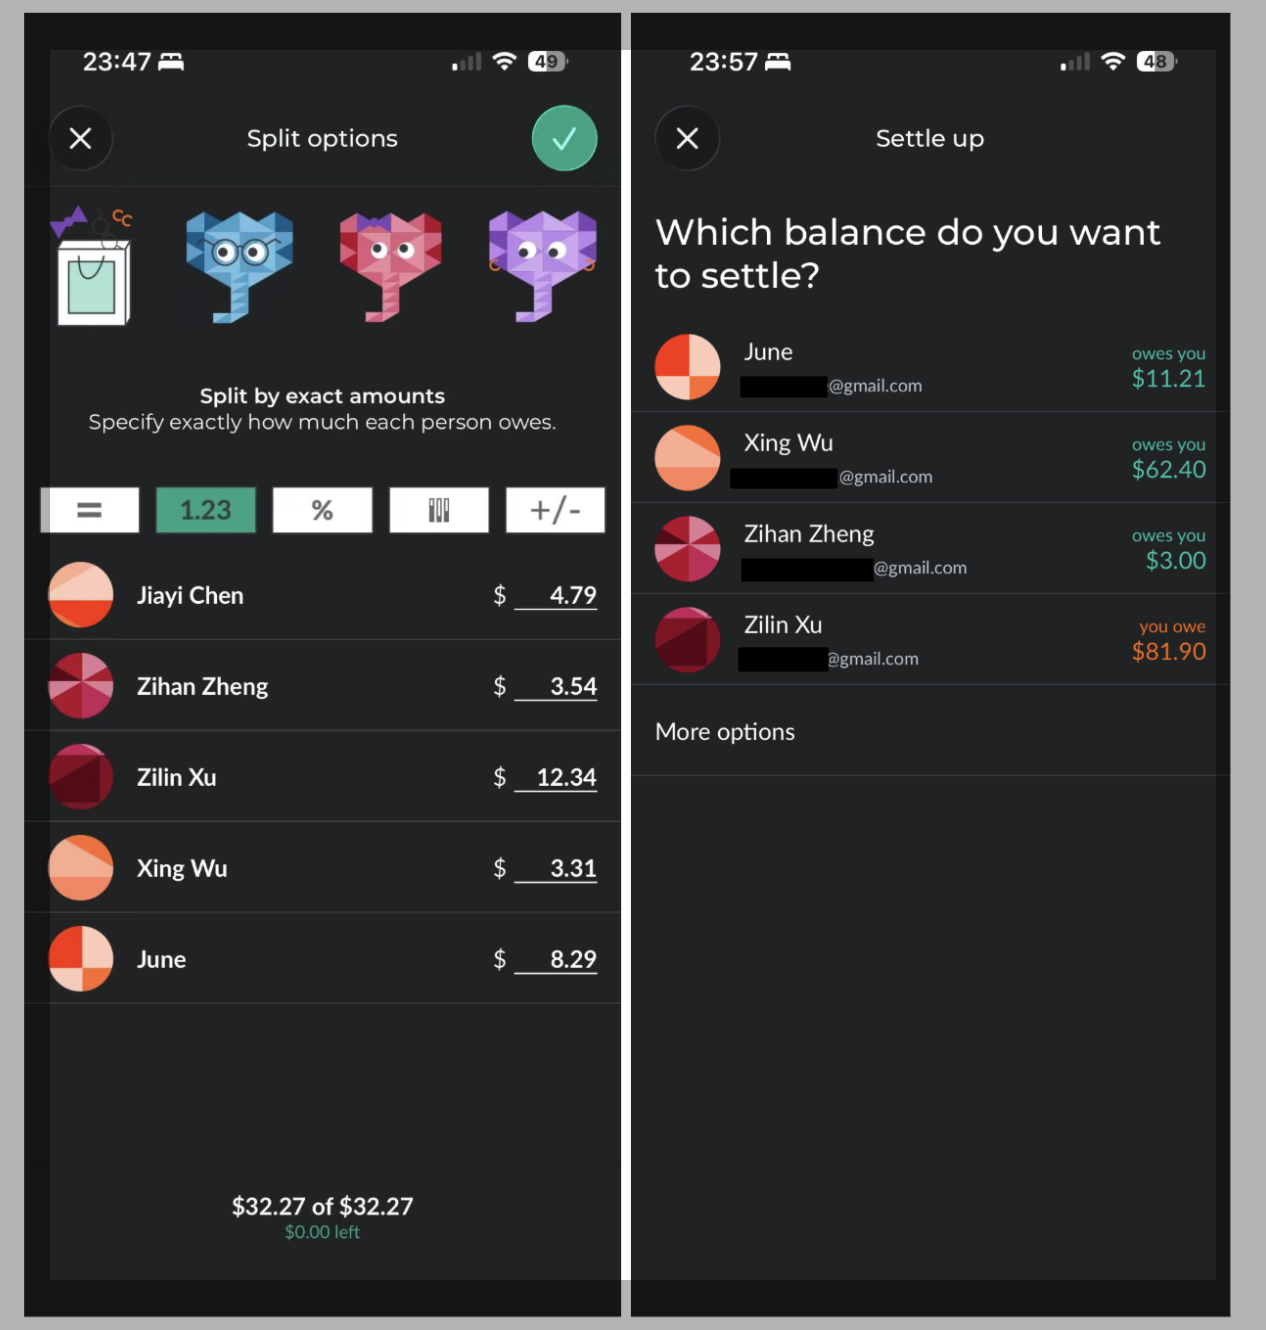
\includegraphics[height=9cm]{Figures/balances_clean.png}
	\caption{Understanding Balances}
	\label{fig:balances_clean}
\end{figure}

\begin{figure}[H]
	\centering
	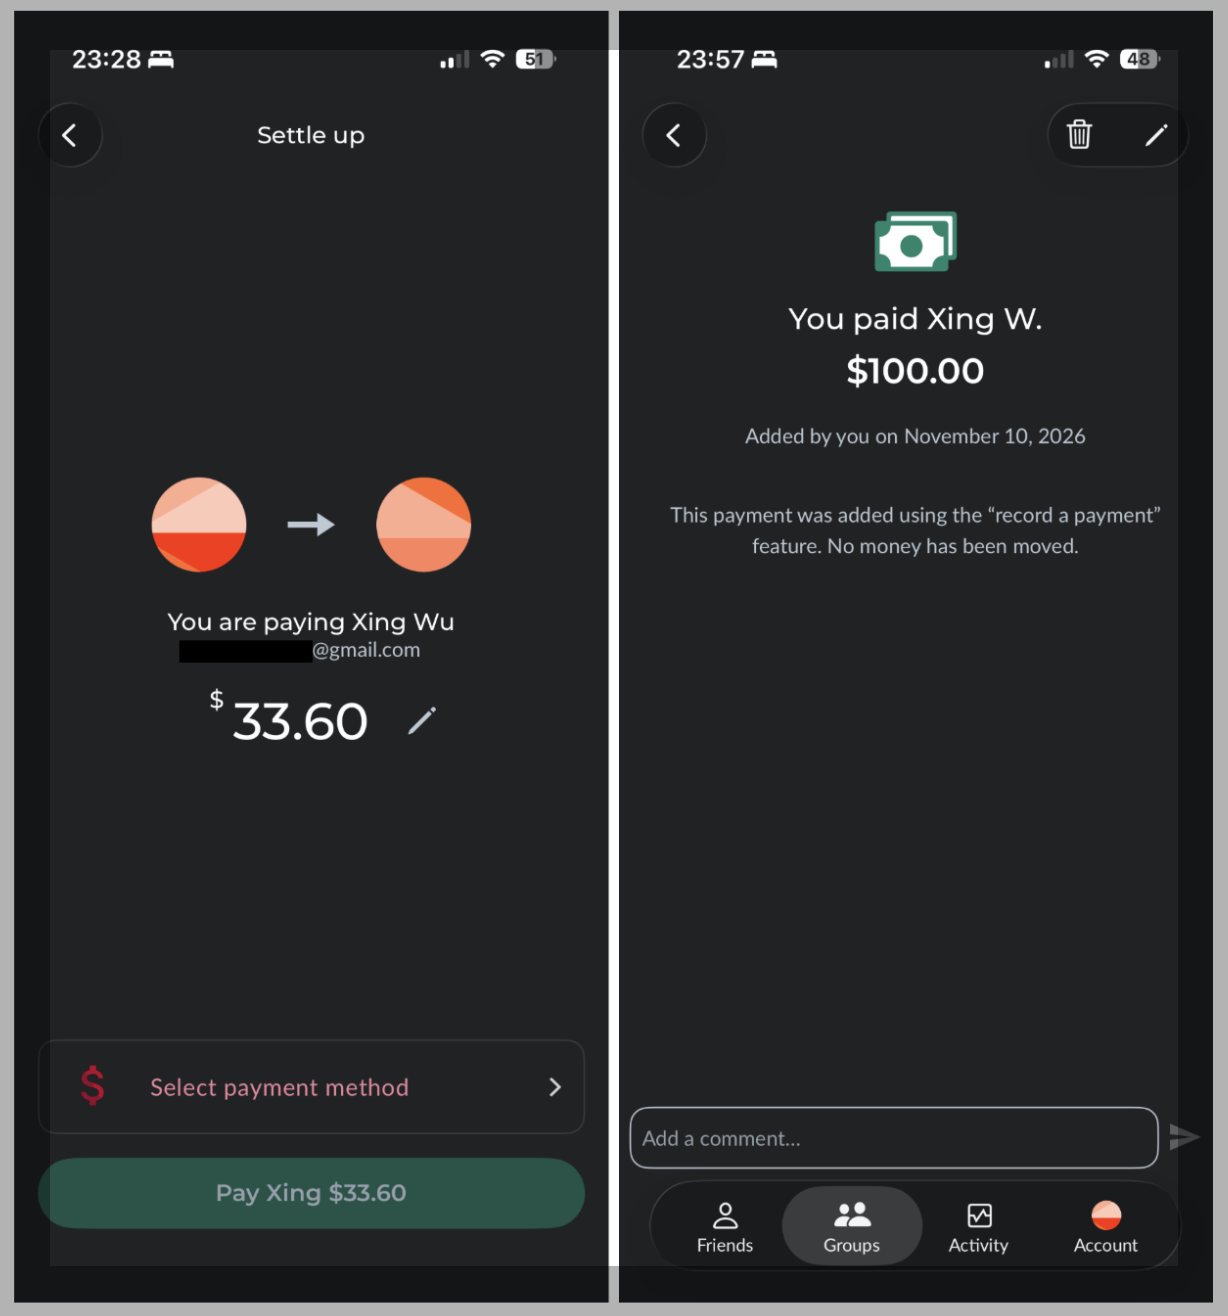
\includegraphics[height=9cm]{Figures/payment_confirmation.png}
	\caption{Payment Confirmation}
	\label{fig:payment_confirmation}
\end{figure}

\begin{figure}[H]
	\centering
	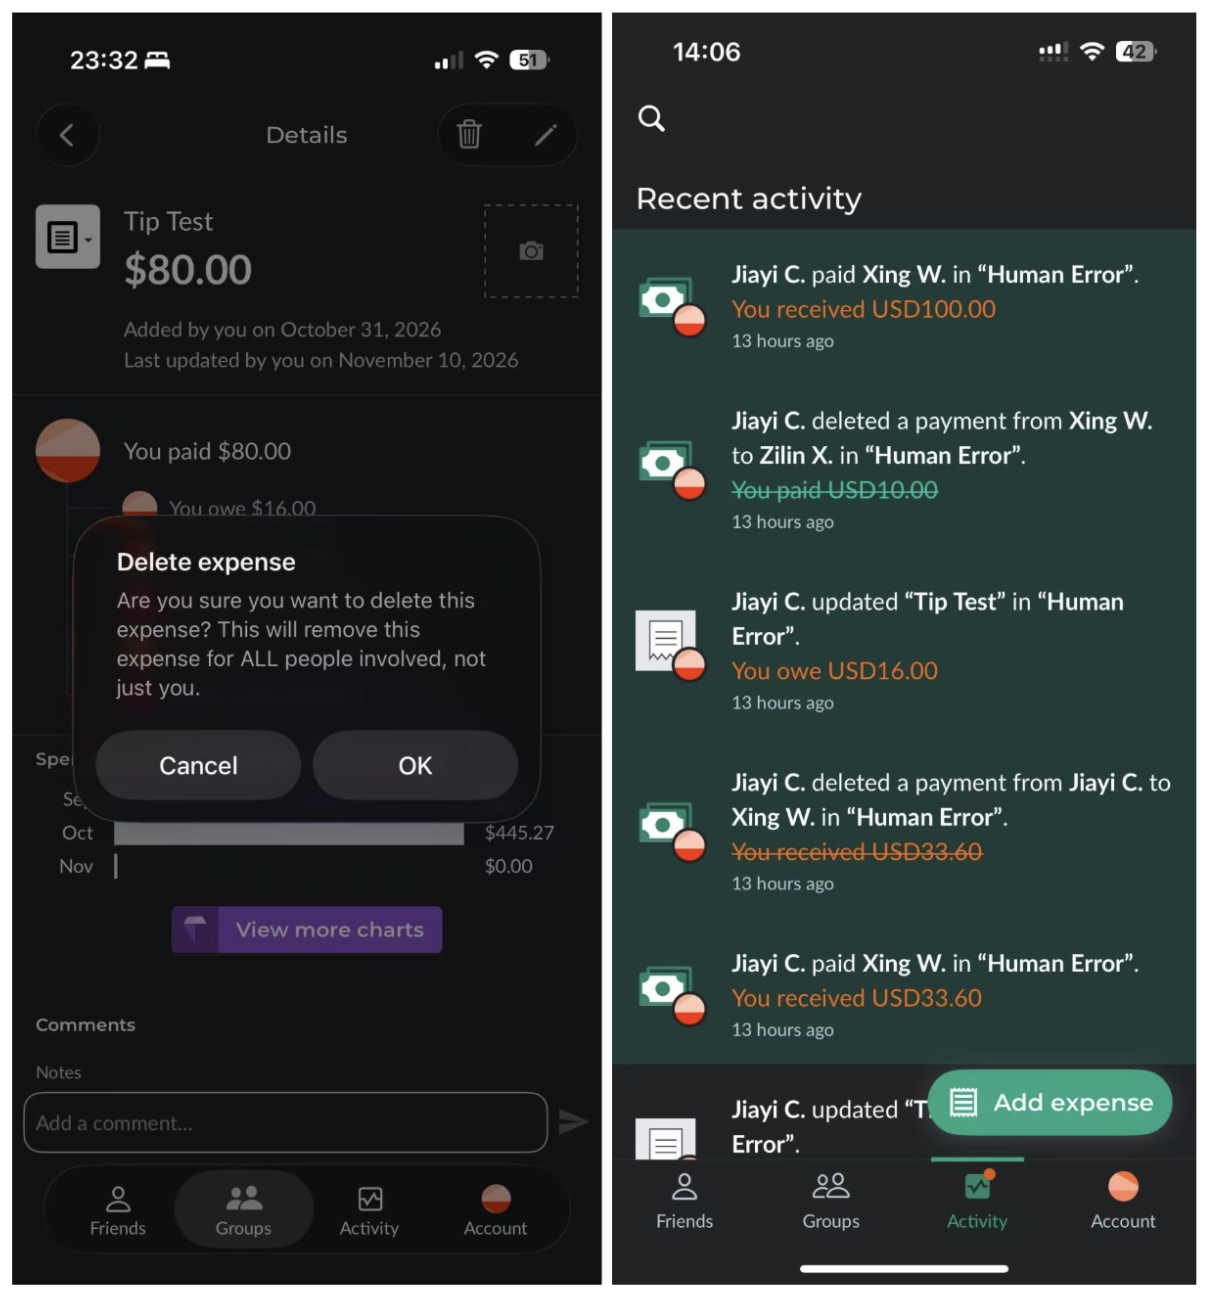
\includegraphics[height=9cm]{Figures/deletion_and_activity.png}
	\caption{Deleting Payments and Activity History}
	\label{fig:eletion_and_activity}
\end{figure}
\section{Product Reviews}
\label{app:reviews}
We collected 50 reviews from the App Store, Google Play, and Trustpilot. The tables below show the categories and a short summary of each review. Review numbers match those used in the Results section. The summaries are written in our own words. Some reviews describe older app versions.

\subsection{Review categories}
We gave each review one main category. Comments mainly about pricing, ads, or entry limits are listed separately from the task findings.

\begin{longtable}{@{}>{\raggedright\arraybackslash}p{3.8in}rr@{}}
\caption{Review categories}\label{tab:categories}\\
\toprule Category & Number & Percentage \\ \midrule
\endfirsthead
\toprule Category & Number & Percentage \\ \midrule
\endhead
\bottomrule\endfoot
Pricing, ads and limits & 26 & 52\% \\
General benefits & 5 & 10\% \\
Understanding amounts & 5 & 10\% \\
Finding and using actions & 3 & 6\% \\
Joining a group & 2 & 4\% \\
Receiving and transferring money & 4 & 8\% \\
Changing shared expenses & 1 & 2\% \\
Receipts and payment options & 2 & 4\% \\
Notifications and communication & 2 & 4\% \\
\midrule
Total & 50 & 100\% \\
\end{longtable}

\subsection{Review records}
The records are kept in their original numbered order so they can be checked against the main text and the Excel file.

\small
\begin{longtable}{@{}p{0.3in}>{\raggedright\arraybackslash}p{1.65in}>{\raggedright\arraybackslash}p{3.3in}>{\raggedright\arraybackslash}p{1.1in}@{}}
\caption{Summary of the 50 reviews}\label{tab:reviews}\\
\toprule No. & User & Review summary & Category \\ \midrule
\endfirsthead
\toprule No. & User & Review summary & Category \\ \midrule
\endhead
\bottomrule\endfoot
1 & @Aaron & Useful for several groups, but the subscription feels expensive. & Pricing, ads and limits \\
2 & madigmcd & Group-trip expenses are easier to manage than in a spreadsheet. & General benefits \\
3 & Tigger Whistler & Likes tracking trip debts and marking payments made outside the app. & General benefits \\
4 & Mirchix & Currency sometimes differs from expectations, so someone must check it. & Understanding amounts \\
5 & I don't love math & Likes receipt scanning and wants to combine payment sources. & Receipts and payment options \\
6 & Where did lists go? & Could not find how to record an outside payment. Support helped. & Finding and using actions \\
7 & ChAaron & Wants receipt recognition from saved photos and iPad split-screen support. & Receipts and payment options \\
8 & danielaCRoberts & Wants to track family expenses without everyone registering. & Joining a group \\
9 & One of the Mels & Wants transaction details and clearer personal versus shared spending totals. & Understanding amounts \\
10 & haizd14 & Still uses Excel to understand where extra costs come from. & Understanding amounts \\
11 & Axeboyrocks & The daily limit prevents entering expenses together at month end. & Pricing, ads and limits \\
12 & Sogeking\_flash & Feels that subscribing has become almost necessary. & Pricing, ads and limits \\
13 & ARon2025 & Plans to stop using the app because of daily limits. & Pricing, ads and limits \\
14 & JenSLi2019 & Accepts ads, but dislikes daily limits and subscription prices. & Pricing, ads and limits \\
15 & Masterofsplitwise & Dislikes the decision to introduce a daily expense limit. & Pricing, ads and limits \\
16 & Br0wn Sug4r & Dislikes limits and waiting timers on basic features. & Pricing, ads and limits \\
17 & Alexdes18 & Likes the idea, but feels practical use requires payment. & Pricing, ads and limits \\
18 & ohhhSimmy & Plans to switch because updates push Pro subscriptions. & Pricing, ads and limits \\
19 & Johnny Martinez & Daily limits get in the way of recording vacation expenses. & Pricing, ads and limits \\
20 & Renisha Shrestha & Uses it a few days monthly; ads and limits interrupt recording. & Pricing, ads and limits \\
21 & Brodyjohn Stancliff & A vague promotional notification reduced trust in the app. & Notifications and communication \\
22 & Auto Vana & Wants a higher free allowance and sees many alternatives. & Pricing, ads and limits \\
23 & Viplav Sharma & Finds limits and selecting percentage splits confusing. & Finding and using actions \\
24 & Stefan & Moved vacation expenses elsewhere after encountering subscription prompts. & Pricing, ads and limits \\
25 & Nevena Milosavljevic & Useful for trips, but daily limits add work. & Pricing, ads and limits \\
26 & Tom C & Likes group splitting, but dislikes annual pricing and prompts. & Pricing, ads and limits \\
27 & ADRIAN & Upgrade prompts make the free version difficult on trips. & Pricing, ads and limits \\
28 & NTG1 & Dislikes annual pricing and reports no advance renewal reminder. & Pricing, ads and limits \\
29 & JONE & Worries about members editing expenses and finds payments difficult. & Changing shared expenses \\
30 & McMenace & Likes the focused app, but worries about shrinking free features. & Pricing, ads and limits \\
31 & Jan Brown & Reports not receiving funds and difficulty getting support. & Receiving and transferring money \\
32 & Mike Sanger & Exports records to Excel because the settlement figures seem unreliable. & Understanding amounts \\
33 & Matt & Annual pricing and free-version interruptions do not suit occasional use. & Pricing, ads and limits \\
34 & Tessa Heyvaert & Switched with housemates because of ads and daily limits. & Pricing, ads and limits \\
35 & Mr E & Previously easy to use, but now feels a subscription is necessary. & Pricing, ads and limits \\
36 & laura taylor & Percentage splits helped three couples share trip expenses. & General benefits \\
37 & Ariel M & Entry limits delayed finishing and settling expenses after a trip. & Pricing, ads and limits \\
38 & Jan M. & Feels daily limits undermine the usefulness of the free version. & Pricing, ads and limits \\
39 & Susan Kemp & Had difficulty splitting on iPhone SE and used paper instead. & Finding and using actions \\
40 & Tommy Koh & Different owing and owed figures caused disagreements among friends. & Understanding amounts \\
41 & Katarina & Finds trip tracking helpful, but only needs it occasionally. & General benefits \\
42 & Kiran & Switched because of waiting timers and daily expense limits. & Pricing, ads and limits \\
43 & CK & Reports missing funds after bank verification and unclear payment status. & Receiving and transferring money \\
44 & Sarah & Dislikes payment changes and the lack of communication about them. & Notifications and communication \\
45 & Steve & Only wants unlimited entries, not the whole premium package. & Pricing, ads and limits \\
46 & Ricky Ricky & Dislikes restrictions on photos and daily entries. & Pricing, ads and limits \\
47 & Daniel Duffill & Finds shared expense recording and settlement easy on app and web. & General benefits \\
48 & Carol & Likes trip splitting and manual records, but payment transfers are slow. & Receiving and transferring money \\
49 & Valerie Salsgiver & Likes splitting costs, but receiving and withdrawing funds takes too long. & Receiving and transferring money \\
50 & Ronnie Cross & Does not know how to create a group without others' contact details. & Joining a group \\
\end{longtable}
\normalsize


\end{document}
